\begin{task}{167}
Пусть \(p\to\infty\), \(s=p!\) и \(n=C_{p^4}^{p^2}\). Найдите функцию~\(f(s)\) в записи \(n=(e+o(1))^{f(s)}\). Здесь \(e=2.71828...\) --- основание натурального логарифма.
\end{task}

\begin{solution}

Выразим \(p\) через \(s\), и наоборот, воспользовавшись формулой Стирлинга:
\begin{gather*}
    s = p! \sim \sqrt{2\pi p} \cdot \left(\frac{p}{e}\right)^p, \\
    \ln{s} \sim \frac{1}{2}\ln{2\pi p} + p\ln{p} - p \sim p\ln{p}, \\
    \ln{\ln{s}} \sim \ln{p} + \ln{\ln{p}} \sim \ln{p}.
\end{gather*}

Получаем \(\displaystyle p \sim \frac{\ln{s}}{\ln{\ln{s}}}\).

Теперь преобразуем \(C_{p^4}^{p^2}, p \rightarrow \infty\):
\begin{multline*}
    C_{p^4}^{p^2} = \frac{(p^4)!}{(p^2)!(p^4 - p^2)!} \sim \frac{\sqrt{2\pi p^4} \left(\frac{p^4}{e}\right)^{p^4}}{\sqrt{2\pi p^2} \left(\frac{p^2}{e}\right)^{p^2}\sqrt{2\pi \left(p^4 - p^2\right)} \left(\frac{p^4 - p^2}{e}\right)^{p^4 - p^2}} = \\
    = \frac{1}{\sqrt{2\pi(p^2 - 1)}} \cdot \frac{(p^2)^{2p^4}}{(p^2)^{p^2}(p^2)^{p^4-p^2}(p^2 - 1)^{p^4-p^2}} = \\
    = \frac{1}{\sqrt{2\pi(p^2 - 1)}} \cdot \frac{(p^2)^{p^4}}{(p^2 - 1)^{p^4-p^2}} \sim 
    \frac{1}{\sqrt{2\pi p^2}} \cdot (p^2)^{p^2}.
\end{multline*}

Последнюю часть преобразований обозначим за \(Q\) и продолжим:
\begin{gather*}
    Q = \frac{1}{\sqrt{2\pi p^2}} \cdot (p^2)^{p^2}, \\
    \ln{Q} = -\frac{1}{2}\ln{2\pi} - \ln{p} + 2p^2\ln{p} \sim 2p^2\ln{p}, \\
    2p^2\ln{p} \sim 2\left(\frac{\ln{s}}{\ln{\ln{s}}}\right)^2 \cdot \ln{\ln{s}} = 2\frac{\ln{s}^2}{\ln{\ln{s}}}.
\end{gather*}

В конечном итоге:
\begin{equation*}
    \ln{C_{p^4}^{p^2}} \sim 2\frac{\ln{s}^2}{\ln{\ln{s}}}.
\end{equation*}

Отсюда можно сделать вывод, что:
\begin{gather*}
    C_{p^4}^{p^2} = (e + o(1))^{2\frac{\ln{s}^2}{\ln{\ln{s}}}} \Rightarrow \\
    \Rightarrow f(s) = 2\frac{\ln{s}^2}{\ln{\ln{s}}}.
\end{gather*}

\textbf{Wolfram} подтвердил, что этот ответ верен (на всякий случай проверил).
\begin{figure}[H]
    \centering
    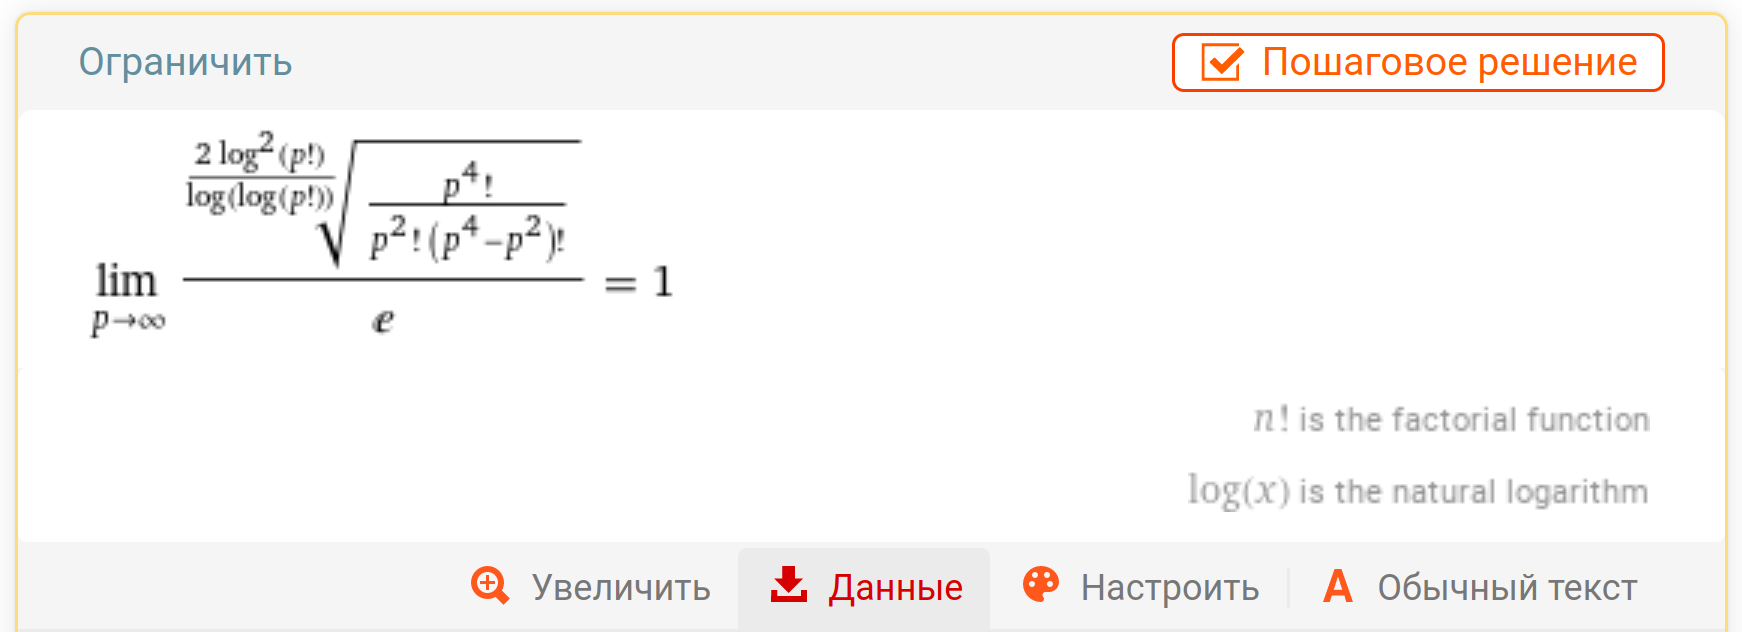
\includegraphics[scale=0.2]{Fall/img/solution-167_confirm.png}
\end{figure}

\textbf{Ответ: } \(\displaystyle f(s) = 2\frac{\ln{s}^2}{\ln{\ln{s}}}\).

\end{solution}
